\documentclass[12pt,a4paper]{report}
\usepackage[top=2.5cm, bottom=2.5cm, left=2.5cm, right=2.5cm]{geometry}

% Diff?rentes options pour la classe :
% - taille de la fonte    : 10pt, 11pt, 12pt
% - recto ou recto-verso    : oneside, twoside
% - stade de d?veloppement    : draft, final


\usepackage[english]{babel}
%\usepackage[latin1]{inputenc}    % Pour utiliser les lettres accentu?es

%\usepackage[utf8]{inputenc}%           gestion des accents (source)
%\usepackage[T1]{fontenc}%              gestion des accents (PDF)
%\usepackage[francais,english]{babel}%          gestion du fran?ais
\usepackage{textcomp}%                 caract?res additionnels
\usepackage[pdftex]{graphicx}
\usepackage{setspace}
\usepackage{hyperref}
\usepackage[english]{varioref}
\usepackage{fancyhdr}
\usepackage{color}
\usepackage{colortbl}
\usepackage{amsmath}
\usepackage{ifpdf} % part of the hyperref bundle
\usepackage{array}
\usepackage[export]{adjustbox}
\usepackage{float}
\usepackage{caption}
\usepackage{tabularx}
\usepackage{tabulary}
\usepackage{enumitem}
\usepackage{courier}
\usepackage[backend=biber, defernumbers=true]{biblatex}
\addbibresource{Webo.bib}
\addbibresource{Biblio.bib}
\DeclareCaptionLabelSeparator{emdash}{\;–\;}

\newcommand{\feature}[1]{\texttt{#1}}

% Increase vertical space between paragraphs for readability
\setlength{\parskip}{0.5\baselineskip}

% Improve spacing inside list environments to avoid dense blocks within items
\setlist[itemize]{itemsep=0.5\baselineskip, parsep=0.5\baselineskip, topsep=0.5\baselineskip}

\captionsetup{
    labelfont={sc},      % Small caps (for FIGURE)
    labelsep=emdash      % Long dash "—" between number and caption
}

%\usepackage{abstract}


 % set fonts for nicer pdf view
 \IfFileExists{lmodern.sty}{\usepackage{lmodern}}{}


\pagestyle{fancy}
\fancyhead[L]{\nouppercase\leftmark} %pour afficher le nom du chapitre ? gauche
\fancyhead[C]{}
\fancyhead[R]{\nouppercase\rightmark} %pour afficher le nom de la section ? droite


\fancyfoot[L]{}
\fancyfoot[C]{}
\fancyfoot[R]{\textbf{\thepage}}

% D?but du document
\begin{document}
%%%%%%%%%%%%% pages de garde en Anglais
\include{garde/garde_fin_English}
\include{garde/garde_sign_fin_English}

\newpage
\pagenumbering{roman}
\chapter*{Dedications}
\addcontentsline{toc}{chapter}{Dedications}
\begin{center}
    \vskip0.5cm
    I dedicate this End-of-Study project
    \vskip0.5cm
    \textbf{To my dear parents}
    \vskip0.2cm
    Dear mother Sawsen and father Elyes, you have been my greatest source of strength throughout this journey. Every sacrifice you have made, every prayer you have offered, and every word of encouragement you have given has brought me to where I am today. I hope to have made you proud, and I know that whatever challenges lie ahead, I will face them with your continuous support.

    \vskip0.5cm
    \textbf{To my dear sisters and brothers}

    \textbf{Oumayma, Eya, Yassmin, Mohamed and Yessin}
    \vskip0.2cm
    Thank you for bearing with me through this period and for all the little things you did they mean to me more than the world. I am truly grateful to have you by my side, and I hope to give back the same love and support you have always given me.

    \vskip0.5cm
    \textbf{To all my family and friends}
    \vskip0.2cm
    To my family, thank you for your warmth and encouragement throughout this journey. To my friends, I may not have always said it, but I am deeply grateful for your presence in my life, and I hope to carry you with me for years to come.
\end{center}
\vskip1cm
\hfill \textbf{Amira BOUAFIF}
\chapter*{Dedication}
\thispagestyle{empty}

\begin{center}
{\large\textit{In the name of Allah, the Most Merciful, the Most Compassionate.}}
\end{center}

\vspace{0.8em}

\noindent I dedicate this work first and foremost to \textbf{Allah}, who is before everything and above everything. No one comes before Him, and nothing would have been possible without His guidance and mercy. The first words revealed to our Prophet Muhammad \raisebox{-0.3em}{
\includegraphics[height=1.2em]{figures/pboh.png}} were \textit{Iqra}, read. This is a reminder of the great value Islam places on knowledge and learning, and of how seeking knowledge is a form of worship and closeness to God.


\noindent\textit{To my dear parents,}\\[0.4em]
All gratitude is to you. I would not be who I am today without your love and sacrifices. From the day I was born until this moment where I stand today, everything I have achieved is because of you. I hope I will always make you proud and honor you the way you deserve.

\vspace{0.7em}

\noindent\textbf{My dear mother}\\[0.3em]
You are a warm, positive, and caring person. Thank you for your endless love, your prayers, and your constant support that gave me strength in every step.

\vspace{0.6em}

\noindent\textbf{My dear father}\\[0.3em]
You have always been by my side in my studies since my earliest years, even from the age of five. Thank you for your patience, your guidance, and your quiet but powerful support that never failed me.


\noindent\textit{To my dear sisters,}\\[0.4em]
\textbf{Asma,} my dear sister, thank you for always being patient with me and for treating me with so much kindness and love.\\[0.4em]
\textbf{Yosr,} my dear sister, thank you for your presence in my life, for your support, and for always being there in your own special way.

\vspace{1em}

\noindent To my grandmother, my uncles, aunts, and cousins, and to all my friends, thank you for your love, encouragement, and support throughout this journey.

\vspace{0.7em}
\begin{center}
\textit{And to everyone who believed in me in any way,}\\[0.3em]
\textit{thank you all.}
\end{center}
\hfill \textbf{Hajer JEMAA}


\chapter*{Acknowledgments}
\addcontentsline{toc}{chapter}{Acknowledgments}
\vskip0.5cm
We would like to extend our sincere gratitude to all those who have supported us throughout the course of this End-of-Study project. Their guidance, encouragement, and support have been invaluable throughout this journey.
\vskip0.5cm
First and foremost, we would like to thank our academic supervisor, Professor Wassim ABBESSI, for his guidance and insights, which have been a great help in the successful completion of this project.
\vskip0.5cm
Our gratitude also go to ITXTREE and, in particular, our professional supervisor, Mr. Firas ABBESSI, for providing us with the opportunity to work on this project and for their professional mentorship.
\vskip0.5cm
we also extend our deep appreciation to the professors at the Higher Institute of Information and Communication Technologies for their invaluable support and teachings, which have greatly contributed to our academic journey.
\vskip0.5cm
Finally, we thank everyone who has, in one way or another, helped in making this project a success.


\tableofcontents    % Table des matières
\listoffigures        % Liste des figures
\listoftables        % Liste des tableaux
\newpage
\pagenumbering{arabic}

\chapter*{General Introduction}
\markboth{General Introduction}{}
\addcontentsline{toc}{chapter}{General Introduction}

In a world where nearly every aspect of life depends on interconnected systems, modern society has become heavily reliant on digital technologies such as communication networks, banking systems, healthcare platforms, transportation systems, and even critical infrastructures.

However, this growing dependence has turned connectivity into a vulnerability to be exploited through cyber attacks, making cybersecurity a necessity.

And in the face of ever-growing and increasingly sophisticated threats, a race began.
Among the many security mechanisms developed to address these threats, Network Intrusion Detection Systems (NIDS) play a critical role.

As the name suggests, NIDS operate at the network level, acting as a key line of defense by monitoring network traffic and detecting malicious activities before they can further propagate into the system.

However, the effectiveness of traditional NIDS has become increasingly challenged by the evolving nature of cyber threats. Built mostly around predefined rules and signatures, these systems remain rigid and reactive, making it difficult for them to keep pace with rapidly changing attack patterns.

Another major concern is reaction time, which remains one of the most critical factors in cybersecurity. The impact of an attack is closely tied not only to how quickly it is detected, but also to how quickly it can be analyzed and responded to. Any delay in this process increases the window of exposure and can significantly amplify its overall impact.  Therefore, minimizing response time becomes essential, something traditional NIDS do not always effectively provide

With the rise of artificial intelligence and its integration into almost every domain, AI emerged as a promising solution to many complex problems, including cybersecurity. By introducing learning and adaptability capabilities.

In this context, Our project focuses on the design and implementation of an AI-based Network Intrusion Detection System.

Throughout this project, we adopt the \textbf{CRISP-DM} methodology \cite{CRISP}.

The first chapter, entitled \textbf{<<Project Context>>}, is devoted to the presentation of the host organization, the analysis of existing solutions, and the definition of the problem statement with the proposed solution.

The second chapter, entitled \textbf{<<Requirements Specification>>}, is dedicated to defining the functional and non-functional requirements, identifying the actors, and modeling the use cases.

The third chapter, \textbf{<<Conceptual Design>>}, presents the conceptual design of the system through the main UML diagrams \cite{UML}.

The fourth chapter, \textbf{<<Data Collection and Preparation>>}, covers data acquisition, data understanding, and data preparation according to the Data Understanding and Data Preparation phases of the CRISP-DM methodology.

The fifth chapter, \textbf{<<Modeling and Evaluation>>}, describes the adopted modeling approach, the training process, and the evaluation of model performance.

The sixth chapter, \textbf{<<Realization>>}, presents model integration, deployment architecture, and the main interfaces of the solution.

Finally, we conclude this report with a general conclusion that summarizes the work carried out, the main contributions, and possible future improvements.
\chapter{Project Context}
%\addcontentsline{toc}{chapter}{}

\section{Introduction}


This chapter serves as an introduction to the project. We begin with a presentation of the company hosting the internship, a study of existing network intrusion detection systems. Then, we present the problem and the proposed solution. Finally, we end the chapter with a conclusion.
\section{Presentation of the company}
ITXTREE is an early-stage technology startup based in Sidi Rzig, Tunisia, focused on building a solid foundation for future digital solutions it is built on the core values of integrity, quality, curiosity and adaptability.
\vskip1cm
\begin{figure}[h!]
    \centering
    \includegraphics[width=0.2\columnwidth]{logos/ITXTREE-logo.png}
\end{figure}

\section{Study of the existing}

\section{Criticism of the existing}

\section{Proposed solution}
Our goal is developing a network intrusion detection system that addresses the identified shortcomings through the following features:

\section{Project Pipeline}
A project pipeline is a structured sequence of stages that outlines the workflow and processes involved in the development and deployment of a project. It serves as a roadmap, guiding the team through various phases, from initial planning to final delivery. 
\vskip0.4cm
Figure~\ref{fig:pipeline} illustrates the project pipeline for our network intrusion detection system.

\begin{figure}[h!]
    \centering
    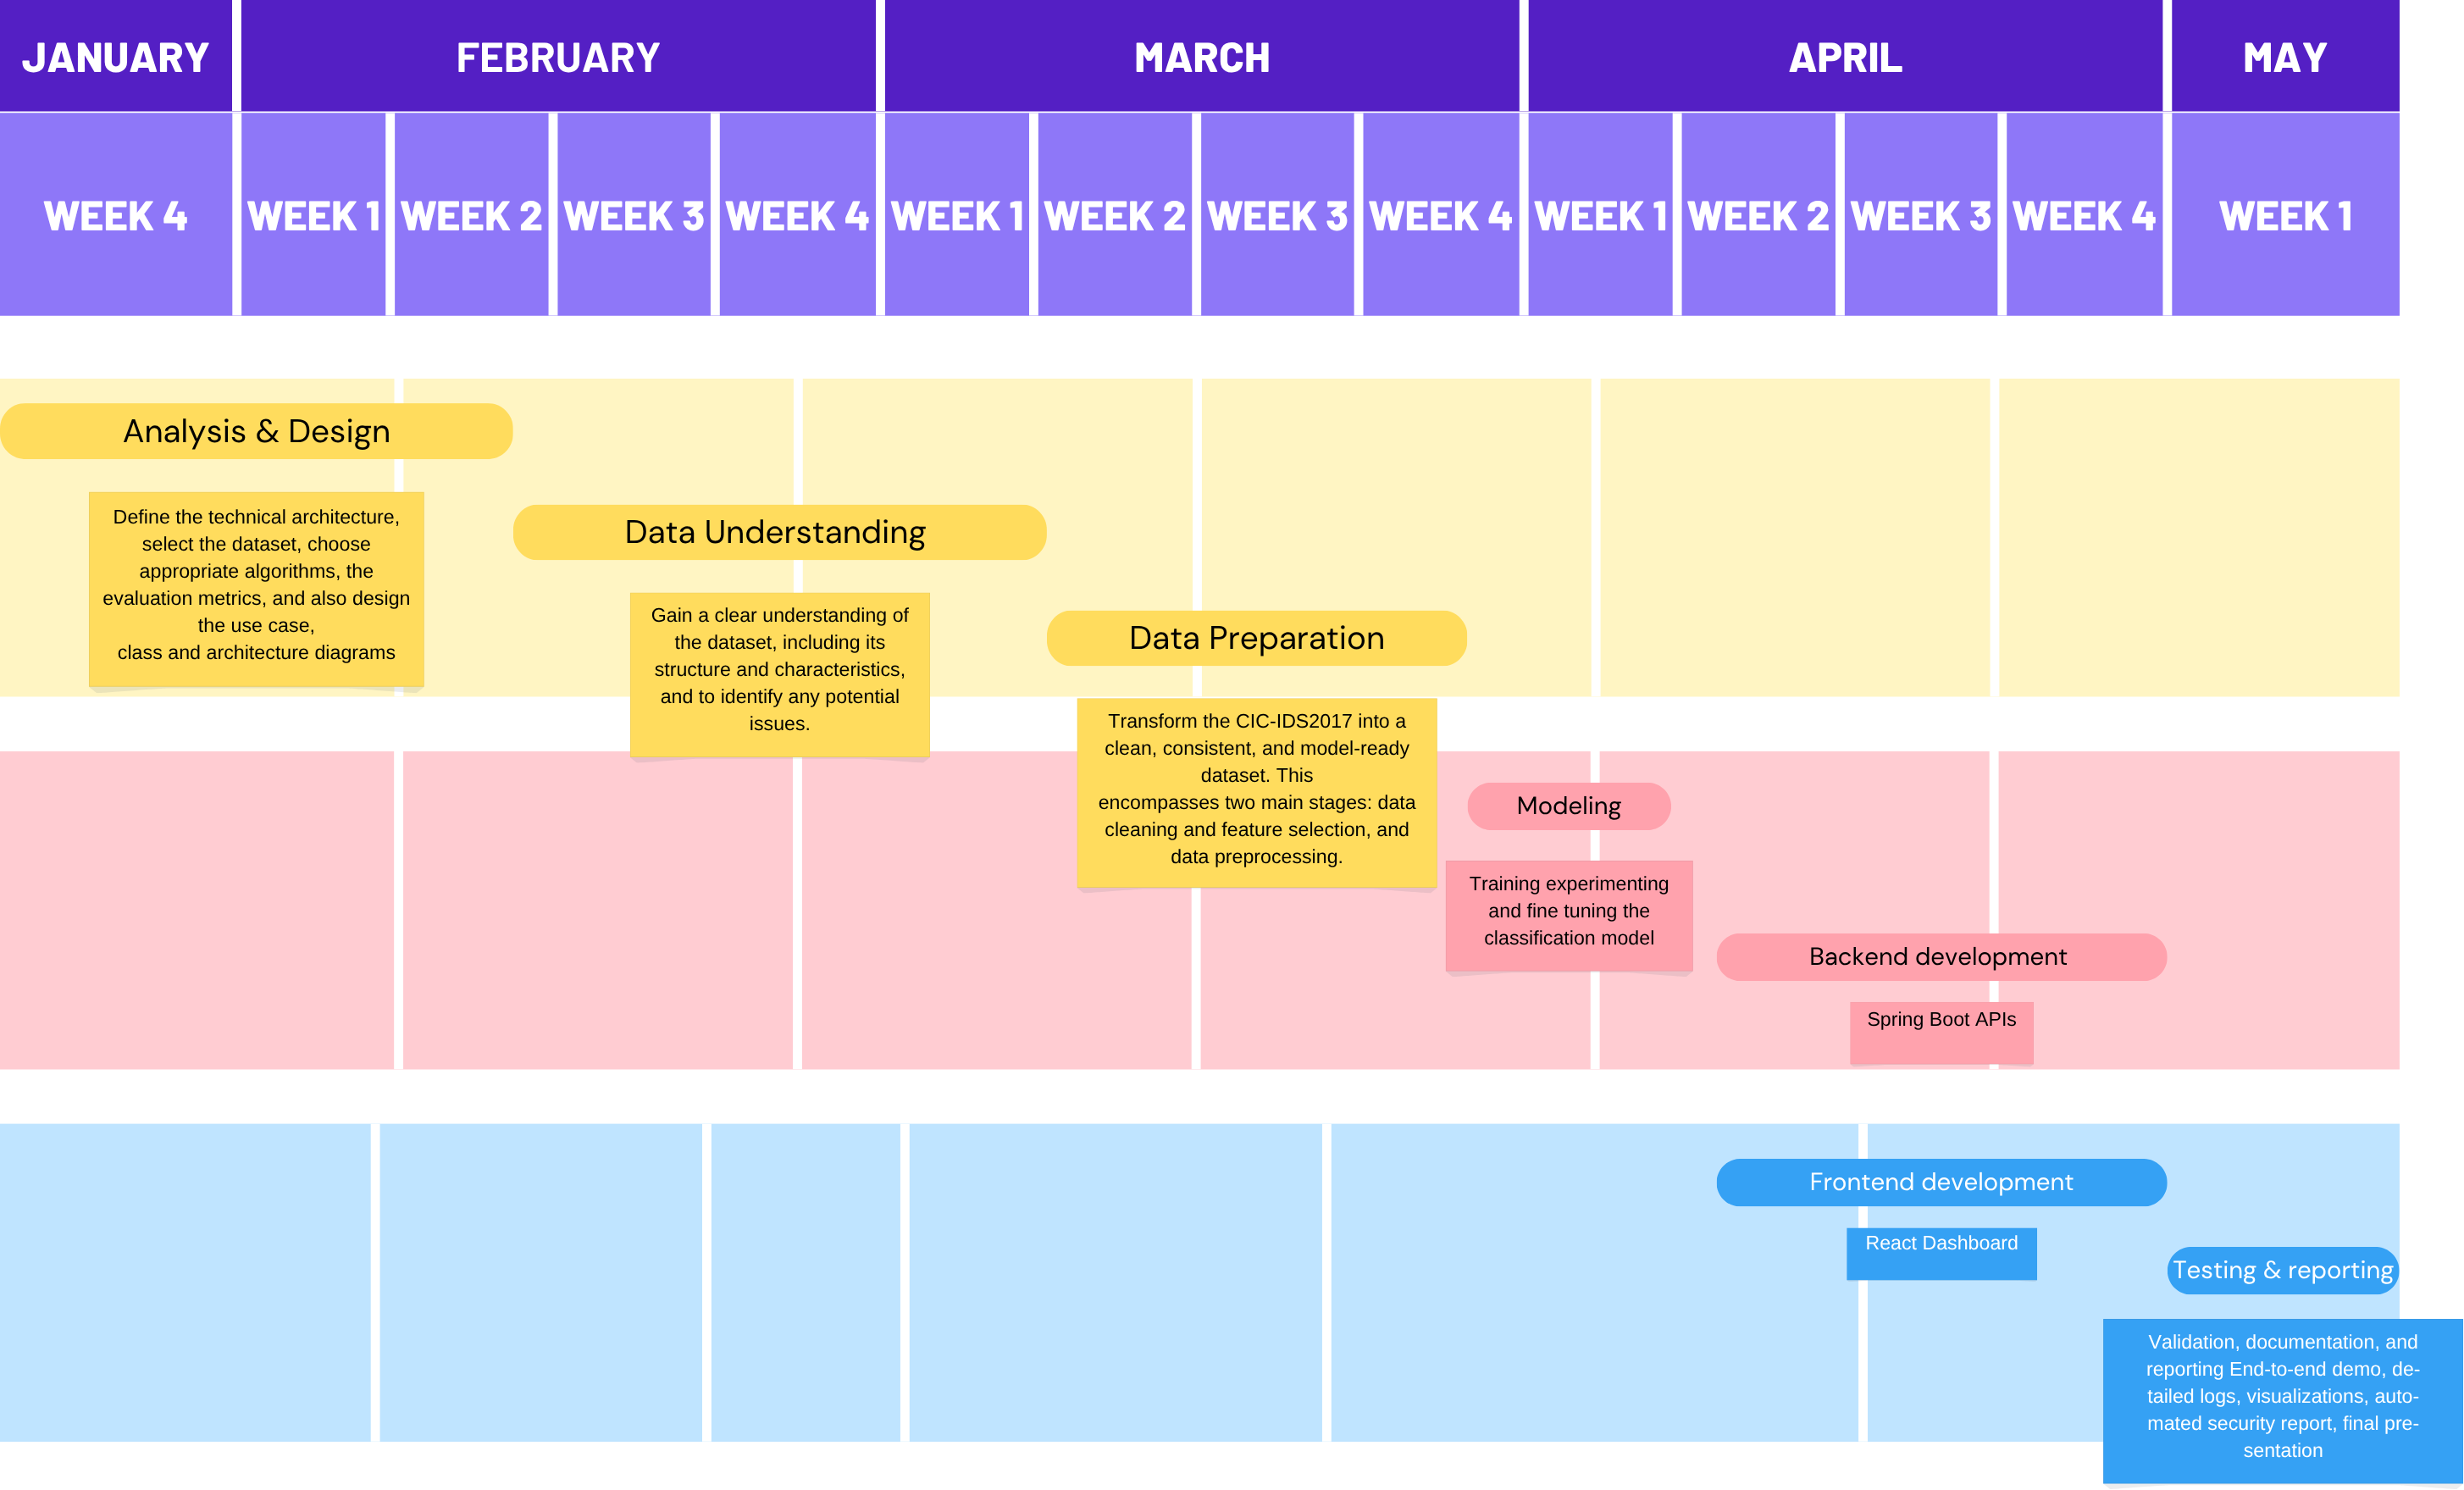
\includegraphics[width=1\columnwidth]{logos/pipeline.png}
    \caption{Project pipeline}
    \label{fig:pipeline}
\end{figure}

\section{Methodologies}
In this section, we present the methodologies that we use in this project, including the machine learning methodology CRISP-DM and the software development methodology UML language.
\newpage
\subsection{CRISP-DM}
The CRISP-DM (Cross-Industry Standard Process for Data Mining) methodology is a widely used framework for structuring machine learning projects. Figure~\ref{fig:crisp-dm} illustrates the six phases of this methodology and their relationships.

\begin{figure}[h!]
    \centering
    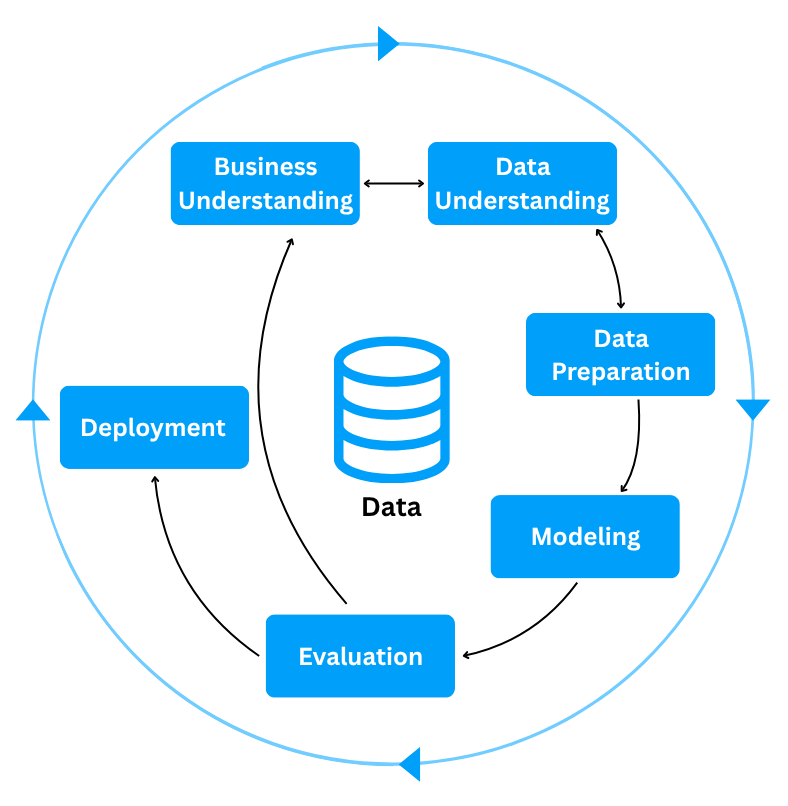
\includegraphics[width=0.6\columnwidth]{logos/CRISP-DM.png}
    \caption{CRISP-DM methodology}
    \label{fig:crisp-dm}
\end{figure}

\subsection{UML Language}
For the modeling of the software system, we use the UML (Unified Modeling Language) language it is a standardized modeling language that helps in specifying, visualizing, constructing, and documenting the artifacts of software systems using diagrams such as use case diagram, class diagram, and sequence diagram.

\begin{figure}[h!]
    \centering
    
\includegraphics[width=0.5\columnwidth]{logos/UML_logo.png}
    \caption{UML language \cite{UML}}
    \label{fig:uml}
\end{figure}

\newpage
\section{Conclusion}
In this chapter we introduce the host company ITXTREE, study existing network intrusion detection systems, discuss their shortcomings and finally present a solution. In the next chapter we specify the system requirements.


\chapter{Requirements Specification}

\section{Introduction}
Throughout this chapter, we specify both the functional and non-functional requirements, identify the system actors, and present the global use case diagram.
By defining these elements, we aim to establish a clear and shared understanding of the system’s expected behavior and constraints, providing a solid foundation for the subsequent design and implementation phases.

\section{Functional Requirements}
Functional requirements define \emph{what} the system should perform. The main functionalities of our system are as follows:

\vskip0.5cm
— Authenticate;
\vskip0.2cm
— View Dashboard;
\vskip0.2cm
— View Statistics summary;
\vskip0.2cm
— Trigger Network Analysis;
\vskip0.2cm
— View Alerts List;
\vskip0.2cm
— View Reports;
\vskip0.2cm
— Analyze Network Flow;

\section{Non-Functional Requirements}

Non-functional requirements define \emph{how} the system should perform its functions. They describe the quality attributes and constraints of the system:

\vskip0.4cm
\textbf{Performance:} The system must process network traffic and generate analysis results with minimal latency, ensuring fast detection of potential intrusions.

\vskip0.3cm
\textbf{Security:} The system must ensure secure authentication and enforce role-based access control, preventing unauthorized actions and protecting system integrity, while supporting non-repudiation to guarantee accountability and traceability of all operations.

\vskip0.3cm
\textbf{Reliability:} The system must perform its functions consistently, handle errors gracefully, and ensure that failures are detected and managed without disrupting overall operation.

\vskip0.3cm
\textbf{Maintainability:} The system should be easy to maintain, allowing for efficient debugging, updates, and modifications to existing components.

\vskip0.3cm
\textbf{Extensibility:} The system should support the addition of new features, such as new detection models or data sources, without requiring major redesign.

\vskip0.3cm
\textbf{Availability:} The system must be accessible and operational whenever needed, minimizing downtime and ensuring continuous monitoring of network activity.

\vskip0.3cm
\textbf{Usability:} The system should provide an intuitive interface, enabling users to efficiently navigate and interact with its functionalities.

\section{Actors Identification}
Actors are external entities, users, organizations, or external systems that interact with the system to achieve one or more functional requirements, with each actor representing a specific role.
\vskip0.05cm
In the context of our project, we identify three primary actors illustrated in Figure~\ref{fig:actors}
\vspace{-0.5cm}
\begin{figure}[h!]
    \centering
    
\includegraphics[width=1\columnwidth]{../diagrams/actors.png}
    \caption{Actors}
    \vspace{-0.5cm}
    \label{fig:actors}
\end{figure}
\vskip0.1cm
Table~\ref{tab3} presents the roles of each actor in our system.
\vspace{-0.1cm}
\begin{table}[H]
    \begin{center}
        \caption{Roles of Actors}
        \label{tab3}
        \begin{tabular}{|l|>{\raggedright\arraybackslash}p{6cm}|}
            \hline
            \rowcolor[gray]{0.8}\bfseries Actor & \bfseries Role             \\
            \hline
            Network/Security                    & - Authenticate             \\
            Administrator                       & - View Dashboard           \\
                                                & - View Statistics Summary  \\
                                                & - Trigger Network Analysis \\
                                                & - View Alerts List         \\
            \hline
            It Manager                          & - Authenticate             \\
                                                & - View Dashboard           \\
                                                & - View Statistics Summary  \\
                                                & - View Reports             \\
            \hline
            Detection Engine                    & - Analyze Network Flow     \\
            \hline
        \end{tabular}
    \end{center}

\end{table}
\newpage
\section{Use Case Diagram}
A use case diagram is a visual representation of \emph{how} users interact with the system and \emph{what} a system does through different use cases.
Figure~\ref{fig:use_case} illustrates that diagram.
\begin{figure}[h!]
    \centering
    
\includegraphics[width=1\columnwidth]{../diagrams/use-case.png}
    \caption{Use Case Diagram}
    \label{fig:use_case}
\end{figure}

\section{Conclusion}
In this chapter, we outline the functional and non-functional requirements of our system, identify the primary actors, and represent the way they interact with the system and the system's functionality via a use case diagram. In the next chapter, we present the conceptual design of the platform.
\chapter{Conceptual Design}
\section{Introduction}
\section{Sequence Diagrams}
\newpage
\section{Class Diagram}
In this section, we present the class diagram of our network intrusion detection system, which is illustrated in Figure \ref{fig:class-diagram}. A class diagram describes the structure of a system by showing the system's classes, their attributes and the relationships among the objects\cite{Class}.
\begin{figure}[h!]
    \centering
    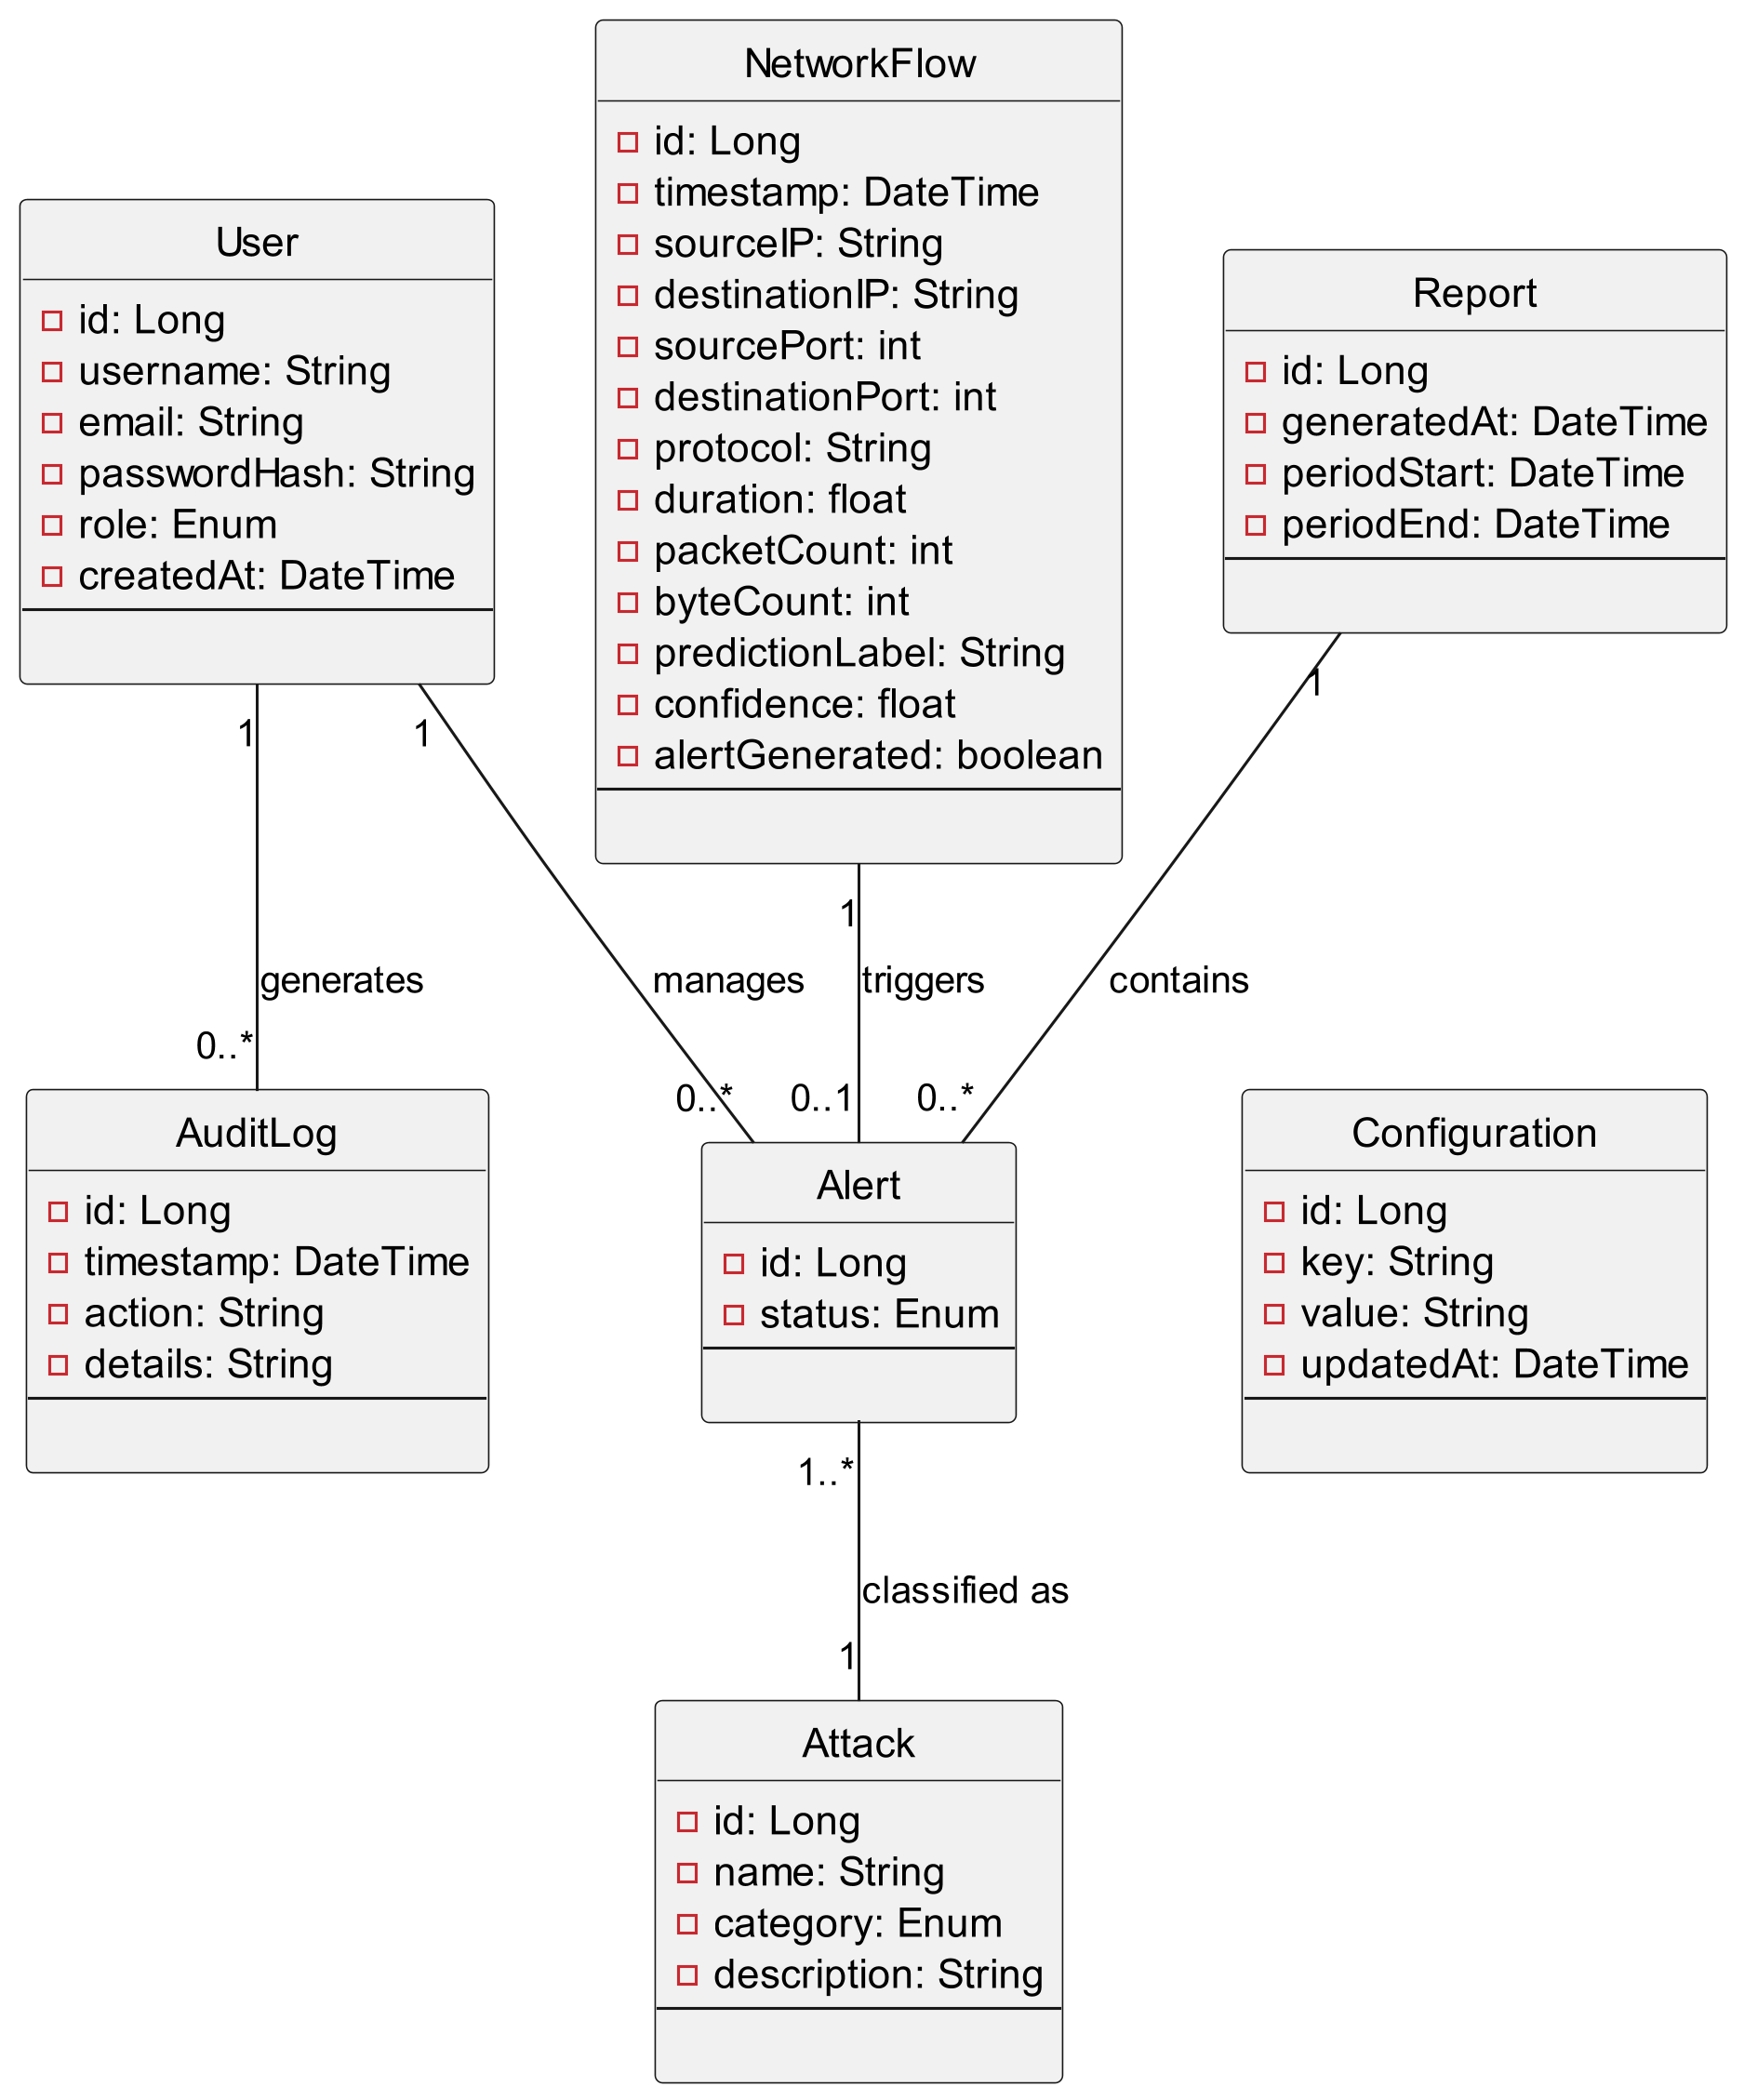
\includegraphics[width=1\columnwidth]{diagrams/class.png}
    \caption{Class Diagram}
    \label{fig:class-diagram}
\end{figure}
\section{Deployment Diagram}
\section{Conclusion}
\chapter{Data Collection and Preparation}

\section{Introduction}

\section{Data Collection}
\newpage
\section{Data Understanding}

The Data Understanding phase of the CRISP-DM methodology focuses on loading, describing, and analyzing the dataset to build a solid foundation for the rest of the project. This section dives into the four tasks of this phase: \texttt{Initial Exploration}, \texttt{Data Description}, \texttt{Data Exploration}, and \texttt{Data Quality}, with each task targeting an aspect of the data, from its structure and content to its quality.

\subsection{Initial Exploration}

The CIC-IDS2017 dataset is captured over five days, it is distributed across 8 files split by day and session: \texttt{Monday}, \texttt{Tuesday}, and \texttt{Wednesday} each corresponding to a single file, while \texttt{Thursday} and \texttt{Friday} are split into AM and PM sessions. The \texttt{Friday PM} session is further divided into two files to isolate the two attacks, \texttt{DDoS} and \texttt{PortScan}.

\subsection{Data Description}
As mentioned in the previous subsection, the dataset is split into 8 files as shown in Table \ref{tab:dataset}.

\begin{table}[H]
    \centering
    \caption{Dataset Files}
    \label{tab:dataset}
    \begin{tabular}{|l|r|r|}
        \hline
        \rowcolor[gray]{0.8} \textbf{File} & \textbf{Number of Rows} & \textbf{Number of Columns} \\
        \hline
        Monday                             & 529,918                 & 79                         \\
        \hline
        Tuesday                            & 445,909                 & 79                         \\
        \hline
        Wednesday                          & 692,703                 & 79                         \\
        \hline
        Thursday AM                        & 170,366                 & 79                         \\
        \hline
        Thursday PM                        & 288,602                 & 79                         \\
        \hline
        Friday AM                          & 191,033                 & 79                         \\
        \hline
        Friday PM (DDoS)                   & 225,745                 & 79                         \\
        \hline
        Friday PM (PortScan)               & 286,467                 & 79                         \\
        \hline
        \textbf{Total}                     & 2,830,743               & ---                        \\
        \hline
    \end{tabular}
\end{table}

The dataset contains a total of 2,830,743 rows across the 8 files. All files have consistent columns, which is expected as they are generated by the same CICFlowMeter pipeline. This consistency allows for seamless concatenation of the files into a single DataFrame for the subsequent analysis.

\vspace{0.5cm}
\begin{itemize}
    \item \textbf{Whitespace Issue:} Leading white spaces is found in columns names and are stripped across all files as they can raise \texttt{KeyError} exceptions when accessing columns by name.
    \item \textbf{Corrupted Labels:} Corrupted labels are discovered in the Thursday AM file, where three labels (\texttt{Web Attack ? Brute Force}, \texttt{Web Attack ? XSS}, \texttt{Web Attack ? Sql Injection}) contain mojibake character instead of en dash (-), and are therefore corrected.
\end{itemize}
These fixes are purely cosmetic and do not alter the underlying data values.
\vspace{0.5cm}

\begin{itemize}
    \item \textbf{Feature Description:} The dataset contains 79 columns, of them 78 are numeric level-flow features and the last one is the target Label. These features can be grouped into 12 categories as shown in Table \ref{tab:features}.
          \begin{longtable}{|p{4cm}|p{6cm}|p{6cm}|}
              \caption{Feature Groups} \label{tab:features}\\
              \hline
              \rowcolor[gray]{0.8} \textbf{Group}                                                                                                                                                                                                                                                                    & \textbf{Features}                                                                                                                                                                              & \textbf{Description}                                                            \\
              \hline
              \endfirsthead
              Flow Metadata                                                                                                                                                                                                                                                                                          &
              \texttt{Destination Port}, \texttt{Flow Duration}                                                                                                                                                                                                                                                      & Total duration of the flow and the destination port                                                                                                                                                                                                                              \\
              \hline
              Packet/Byte Count                                                                                                                                                                                                                                                                                      &
              \texttt{Total Fwd Packets}, \texttt{Total Backward Packets}, \texttt{Total Length of Fwd Packets}, \texttt{Total Length of Bwd Packets}, \texttt{act\_data\_pkt\_fwd}                                                                                                                                  & Number of packets and packet bytes in both forward (from source to destination) and backward directions (from destination to source), and packets having actual data in the forward direction.                                                                                   \\
              \hline
              Packet/Segment Length Statistics                                                                                                                                                                                                                                                                       &
              \texttt{Fwd Packet Length Max/Min/Mean/Std}, \texttt{Bwd Packet Length Max/Min/Mean/Std}, \texttt{Max/Min Packet Length}, \texttt{Packet Length Mean/Std/Variance}, \texttt{Average Packet Size}, \texttt{Avg Fwd Segment Size}, \texttt{Avg Bwd Segment Size}                                         & Packets and segments length statistics (e.g. max, min, mean, std etc...).
              \\
              \hline
              Flow Rate                                                                                                                                                                                                                                                                                              &
              \texttt{Flow Bytes/s}, \texttt{Flow Packets/s}, \texttt{Fwd Packets/s}, \texttt{Bwd Packets/s}, \texttt{Down/Up Ratio}                                                                                                                                                                                 & Flow throughput, forward and backward packet rates, flow asymmetry ratio (backward packets (download) to forward packets (upload)).
              \\
              \hline
              Inter-Arrival Time                                                                                                                                                                                                                                                                                     & \texttt{Flow IAT Max/Min/Mean/Std}, \texttt{Fwd IAT Max/Min/Mean/Std/Total}, \texttt{Bwd IAT Max/Min/Mean/Std/Total}                                                                           & Time between consecutive packets in the flow, forward, and backward directions.
              \\
              \hline
              TCP Flag Count                                                                                                                                                                                                                                                                                         &
              \texttt{FIN Flag Count}, \texttt{SYN Flag Count}, \texttt{RST Flag Count}, \texttt{PSH Flag Count}, \texttt{ACK Flag Count}, \texttt{URG Flag Count}, \texttt{CWE Flag Count}, \texttt{ECE Flag Count}, \texttt{Fwd PSH Flags}, \texttt{Bwd PSH Flags}, \texttt{Fwd URG Flags}, \texttt{Bwd URG Flags} & TCP flags counts for the entire flow, forward and backward directions.                                                                                                                                                                                                           \\
              \hline
              Header Length                                                                                                                                                                                                                                                                                          &
              \texttt{Fwd Header Length}, \texttt{Bwd Header Length}, \texttt{Fwd Header Length.1}                                                                                                                                                                                                                   & Backward and forward header lengths.                                                                                                                                                                                                                                             \\
              \hline
              Bulk Transfer Statistics                                                                                                                                                                                                                                                                               &
              \texttt{Fwd Avg Bytes/Bulk}, \texttt{Fwd Avg Packets/Bulk}, \texttt{Fwd Avg Bulk Rate}, \texttt{Bwd Avg Bytes/Bulk}, \texttt{Bwd Avg Packets/Bulk}, \texttt{Bwd Avg Bulk Rate}                                                                                                                         & Average forward and backward bulk (a sequence of consecutive packets in the same direction) transfer statistics.                                                                                                                                                                 \\
              \hline
              Subflow Packet/Byte Count                                                                                                                                                                                                                                                                              &
              \texttt{Subflow Fwd Packets}, \texttt{Subflow Fwd Bytes}, \texttt{Subflow Bwd Packets}, \texttt{Subflow Bwd Bytes}                                                                                                                                                                                     & Number of packets and packet bytes in both directions in a subflow.                                                                                                                                                                                                              \\
              \hline
              Window/Segment Size                                                                                                                                                                                                                                                                                    &
              \texttt{Init\_Win\_bytes\_forward}, \texttt{Init\_Win\_bytes\_backward}, \texttt{min\_seg\_size\_forward}                                                                                                                                                                                              & Window sizes in both the forward and backward directions and the minimal segment size in the forward direction.                                                                                                                                                                  \\
              \hline
              Active/Idle Time                                                                                                                                                                                                                                                                                       &
              \texttt{Active Max/Min/Mean/Std}, \texttt{Idle Max/Min/Mean/Std}                                                                                                                                                                                                                                       & Duration of active and idle periods within a flow.                                                                                                                                                                                                                               \\
              \hline
              Target                                                                                                                                                                                                                                                                                                 &
              \texttt{Label}                                                                                                                                                                                                                                                                                         & The target label indicating the class the flow belongs to.
              \\
              \hline
          \end{longtable}
          \begin{itemize}
              \item \textbf{Duplicate Column:} The column \texttt{Fwd Header Length.1} is identified as a duplicate of \texttt{Fwd Header Length}, confirmed by the fact that both contain the same values.
              \item \texttt{Packet Length Mean} and \texttt{Average Packet Size} both measure the average packet size, but the two do not hold the same values as they are calculated differently: the former uses the statistical mean, while the latter divides the total length of packets by the total number of packets\cite{CICFlowMeter}.
          \end{itemize}
\end{itemize}

All 54 features are of type \texttt{int64}, 24 features are of type \texttt{float64}, with the last feature, the target \emph{Label}, being of type \texttt{object}.

\vspace{0.5cm}
Table \ref{tab:feature_stat} presents the statistics of some of the features.
\begin{table}[H]
    \centering
    \caption{Feature Statistics}
    \label{tab:feature_stat}
    \begin{tabular}{|l|r|r|r|r|}
        \hline
        \rowcolor[gray]{0.8} \textbf{Feature} & \textbf{Min} & \textbf{Max} & \textbf{Mean} & \textbf{Std} \\
        \hline
        Flow Duration        &  -13   &   119,999,998    &  14,785,663.92   & 33,653,744.09 \\
        \hline
        Total Backward 
        Packets    &  0    &  121,922   & 10.39   &  997.39      \\
        \hline
        act\_data\_pkt fwd   &  0     &  213,557    &  5.42  &     636.43   \\
        \hline
        Min Packet Length  & 0  & 1,448  & 16.43 & 25.24 \\
        \hline
        Flow Bytes/s  & -241,000,000  & inf  & inf  & inf \\
        \hline
        Flow IAT Max & -13 & 120,000,000  &  9,182,475.32  & 24,459,539.25 \\
        \hline
        Bwd PSH Flags  &  0 & 0 & 0 & 0 \\
        \hline
        Fwd Header Length  & -322,212,234,632  &  4,644,908  &  -25,997.39  & 21,052,857.87 \\
        \hline
        Bwd Avg Bulk Rate & 0 &  0 & 0 & 
        0 \\
        \hline
    \end{tabular}
\end{table}

Some of the feature has negative, inf and constant statistic of zero. Those features are further investigated in the data quality section.
\begin{itemize}
    \item \textbf{Class Distribution:} The dataset contains 15 classes, BENIGN and 14 attacks, Table \ref{tab:classes} shows the distribution of these classes across the dataset files.
    \newpage
          \begin{longtable}{|l|l|r|}
              \caption{Class Distribution}\label{tab:classes}                                        \\
              \hline
              \rowcolor[gray]{0.8} \textbf{File} & \textbf{Class}             & \textbf{Class Count} \\
              \hline
              Monday                             & BENIGN                     & 529,918              \\
              \hline
              \multirow{3}{*}{Tuesday}
                                                 & BENIGN                     & 432,074              \\
              \cline{2-3}
                                                 & FTP-Patator                & 7,938                \\
              \cline{2-3}
                                                 & SSH-Patator                & 5,897                \\
              \hline
              \multirow{6}{*}{Wednesday}
                                                 & BENIGN                     & 440,031              \\
              \cline{2-3}
                                                 & DoS Hulk                   & 232,443              \\
              \cline{2-3}
                                                 & DoS GoldenEye              & 10,293               \\
              \cline{2-3}
                                                 & DoS Slowloris              & 5,796                \\
              \cline{2-3}
                                                 & DoS Slowhttptest           & 5,499                \\
              \cline{2-3}
                                                 & Heartbleed                 & 11                   \\
              \hline
              \multirow{4}{*}{Thursday AM}
                                                 & BENIGN                     & 168,186              \\
              \cline{2-3}
                                                 & Web Attack - Brute Force   & 1,507                \\
              \cline{2-3}
                                                 & Web Attack - XSS           & 652                  \\
              \cline{2-3}
                                                 & Web Attack - Sql Injection & 21                   \\
              \hline
              \multirow{2}{*}{Thursday PM}
                                                 & BENIGN                     & 288,566              \\
              \cline{2-3}
                                                 & Infiltration               & 36                   \\
              \hline
              \multirow{2}{*}{Friday AM}
                                                 & BENIGN                     & 189,067              \\
              \cline{2-3}
                                                 & Bot                        & 1,966                \\
              \hline
              \multirow{2}{*}{Friday PM (DDoS)}
                                                 & DDoS                       & 128,027              \\
              \cline{2-3}
                                                 & BENIGN                     & 97,718               \\
              \hline
              \multirow{2}{*}{Friday PM (PortScan)}
                                                 & PortScan                   & 158,930              \\
              \cline{2-3}
                                                 & BENIGN                     & 127,537              \\
              \hline
          \end{longtable}
\end{itemize}

With the exception of Monday, which contains only BENIGN traffic, all files contain at least one attack class alongside BENIGN samples. Each attack class is present in only one file. 

Table \ref{tab:attack_classes} provides a description of the 14 attack classes of the dataset.

\begin{longtable}{|p{3.5cm}|p{11.5cm}|}
    \caption{Attack Classes}\label{tab:attack_classes} \\
    \hline
    \rowcolor[gray]{0.8}\textbf{Class}                    & \textbf{Description} \\
    \hline
    \endfirsthead

    \vfill
    \textbf{FTP-Patator} (File Transfer Protocol Patator) &
    \vspace{0.05cm}
    A brute force attack using the Patator tool targeting FTP servers, an old unencrypted protocol that transmits data and credentials in plain text, using trial and error to guess credentials in order to gain unauthorized access.
    \vspace{0.5cm}
    \\
    \hline

    \vfill
    \textbf{SSH-Patator} (Secure Shell Patator)           &
    \vspace{0.05cm}
    A brute force attack using the Patator tool targeting SSH servers, a secure encrypted protocol that encrypts the entire session including the login, using trial and error to gain unauthorized access to individual accounts.
    \vspace{0.5cm}
    \\
    \hline

    \vfill
    \textbf{DoS Hulk}                                     &
    \vspace{0.05cm}
    A Denial-of-Service attack using the HULK tool, which is used to overwhelm web servers by generating a large number of unique randomized requests at irregular intervals.
    \vspace{0.5cm}
    \\
    \hline

    \vfill
    \textbf{DoS GoldenEye}                                &
    \vspace{0.05cm}
    A Denial-of-Service attack using the GoldenEye tool, which dynamically generates multiple parallel connections (multi-threaded) to a target URL while keeping them alive to exhaust the available connection slots, simultaneously forcing the server to bypass caching mechanisms and fully process every request.
    \vspace{0.5cm}
    \\
    \hline

    \vfill
    \textbf{DoS slowloris}                                &
    \vspace{0.05cm}
    A Denial-of-Service attack using the Slowloris tool, which enables a single machine to overwhelm a web server by opening multiple connections and keeping them open by sending partial requests (only headers) periodically, while requiring very low bandwidth, hence its name, as it operates in a low and slow manner.
    \vspace{0.5cm}
    \\
    \hline

    \vfill
    \textbf{DoS Slowhttptest}                             &
    \vspace{0.05cm}
    A Denial-of-Service attack using the SlowHTTPTest tool, which creates very slow connections by sending seemingly legitimate requests using low bandwidth and intentionally delaying their completion, thereby consuming the limited number of concurrent connections the server can handle.
    \vspace{0.5cm}
    \\
    \hline

    \vfill
    \textbf{Heartbleed}                                   &
    \vspace{0.05cm}
    An attack in which the attacker exploits the Heartbleed bug in the OpenSSL cryptographic library to read sensitive memory contents by sending malformed heartbeat requests demanding more memory than the actual payload from the server running the vulnerable version of OpenSSL, after which the server allocates the requested memory without any verification and returns it, exposing whatever sensitive data happened to be stored in that memory chunk at that moment. It is used to steal private encryption keys, usernames and passwords, and to intercept session tokens, permitting session hijacking by providing the stolen token to the server so that the attacker is treated as a legitimate logged-in user, as well as to decrypt previously captured encrypted traffic that the attacker had intercepted beforehand.
    \vspace{0.5cm}
    \\
    \hline

    \vfill
    \textbf{Web Attack - Brute Force}                     &
    \vspace{0.05cm}
    An attack that uses a forceful approach to steal credentials to gain unauthorized access to systems. It can be carried out in many ways, from trying common credential combinations manually, to using dictionary attacks, or a combination of both.
    \vspace{0.5cm}
    \\
    \hline

    \vfill
    \textbf{Web Attack - XSS}                             &
    \vspace{0.05cm}
    An attack in which malicious scripts are injected into trusted websites, by exploiting their input validation vulnerability, and executed by other end users' browsers, which have no way to distinguish it from legitimate content.
    \vspace{0.5cm}
    \\
    \hline

    \vfill
    \textbf{Web Attack - Sql Injection}                   &
    \vspace{0.05cm}
    An attack in which the attacker interferes with the queries that an application makes to its database enabling him to view data that he is not supposed to have access to, including data belonging to other users and any other data that the platform has access to, as well as modify or delete it. It is carried out by injecting malicious SQL queries into an input field, which the vulnerable application passes directly to the database as a query instead of treating it as plain data. The database then executes it, allowing the attacker to manipulate the database in unintended ways.
    \vspace{0.5cm}
    \\
    \hline

    \vfill
    \textbf{Infiltration}                                 &
    \vspace{0.05cm}
    A multi-stage attack to gain unauthorized access to systems, in which the attacker first deploys a malicious file disguised as a legitimate one, such as a document or a downloadable link, containing a backdoor. The victim executes the file unknowingly, after which the backdoor establishes a reverse connection back to the attacker's machine, granting the attacker remote control over the compromised system. Once inside, the attacker scans the victim's internal network using tools (e.g. Nmap) to discover live hosts (any active and reachable device on the network), as well as open ports and running services. This allows the attacker to map the internal network and identify potential targets for further infiltration. The attacker then moves laterally by infiltrating another machine, spreading the attack further across the network. Finally, an attempt is made to exfiltrate sensitive data (transferring confidential information out of the network), and to escalate privileges on the compromised systems in order to gain access to even more restricted and sensitive resources.
    \vspace{0.5cm}
    \\
    \hline

    \vfill
    \textbf{Bot}                                          &
    \vspace{0.05cm}
    An attack carried out using the ARES botnet, a malware-based network of compromised computers built on a RAT (Remote Access Trojan) and botnet framework, which allows the attacker to take control of infected machines and coordinate them for malicious purposes. It first infects victim machines using phishing emails or malicious downloads, after which the infected machines connect back to the attacker's Command and Control (C\&C) server. Finally, the attacker issues commands to all bots, that is, all infected machines, simultaneously.
    \vspace{0.5cm}
    \\
    \hline

    \vfill
    \textbf{DDoS}                                         &
    \vspace{0.05cm}
    An attack used to overwhelm the target system with a flood of traffic from multiple sources, making it unable to respond to legitimate requests, potentially leading to a complete shutdown of the system.
    \vspace{0.5cm}
    \\
    \hline

    \vfill
    \textbf{PortScan}                                     &
    \vspace{0.05cm}
    An attack used to discover open ports and whether they are receiving or sending data, in addition to potential vulnerabilities that could be exploited.
    \vspace{0.5cm}
    \\
    \hline
\end{longtable}


\subsection{Data Exploration}

\section{Data Preparation}

\section{Data Augmentation}

\section{Conclusion}

\chapter{Modeling}

\section{Introduction}

\section{State of the Art}

\section{Adopted Approach}

\section{Training and Hyperparameter Optimization}

\section{Conclusion}

\chapter{Realization}

\section{Introduction}

\section{Development Tools and Technologies}

\section{Performance Analysis and Evaluation Metrics}

\section{User Interfaces}

\section{Integration}

\section{Conclusion}

\chapter*{General Conclusion}
\markboth{General Conclusion}{}
\addcontentsline{toc}{chapter}{General Conclusion}
This project focused on building an AI-based intrusion detection system
The work was structured around several main stages. We first defined the project context and justified the choice of an AI-driven approach by highlighting the weaknesses of traditional signature-based systems. We then specified the requirements, identified the actors and modeled the system, before moving to data collection and preparation, which proved to be one of the most demanding phases of the project. Finally, we carried out the modeling, evaluation, and realization steps in order to transform the research work into an operational solution.

Among the most important findings of this project was the fact that performance in intrusion detection depends as much on data quality as on algorithmic choice. The CIC-IDS2017 dataset offered a rich and realistic basis for experimentation, but it also required extensive inspection and preprocessing due to corrupted values, duplicated records, contradictory samples, and features affected by extraction issues. This stage confirmed that in any data science project, the reliability of the input data is often a decisive factor in the quality of the final model.

Some objectives, however, could not be completed within the available time. In particular, we were unable to implement the transformation pipeline that would convert raw PCAP files captured in real time into a ready for prediction dataset row. This step was intentionally postponed due to its complexity and because of the feature extraction process itself. Especially that CICFlowMeter, showed instability and bugs during the data understanding phase. With more time, we would have designed and integrated this pipeline to obtain a more complete end-to-end system.

As a future extension, the most promising direction would be to add a deep learning layer trained on a suitable dataset. Such an addition could enrich the current solution by capturing more complex patterns and improving the system's ability to detect sophisticated or evolving attacks. It would also open the way to a more advanced hybrid architecture, combining the strengths of classical machine learning with deeper representation learning.

Overall, this project provided a practical experience in designing and implementing an AI-based intrusion detection system, highlighting both the potential and limitations of this approach.


\printbibliography[title={Webography}, keyword=web, resetnumbers=true]
\printbibliography[title={Bibliography}, notkeyword=web, resetnumbers=true]

% Fin du document
\end{document}